%\newlist{todolist}{itemize}
%\setlist[todolist]{label=$\square$}


\chapter{Checkliste zum Studiumsbeginn}

\Large



\begin{itemize}[label=$\square$]
	
	\item Immatrikuliert sein
	\item Campuscard validieren
	\item Bafög-Antrag stellen
	\item Wohnsitz ummelden
	\item GEZ anmelden
	\item (Optional) Deutschlandticket abonnieren
	\item sich in HeiCO (\autopageref{digitale-tools-uebersicht}) für Vorlesungen und Übungen zu Vorlesungen anmelden
	\item sich in Übungsgruppen zu den Vorlesungen eintragen (Physik-Übungsgruppen-System, MaMpf, Moodle)
	\item Zettelpartner finden
\end{itemize}

\begin{figure}[b]
	\centering
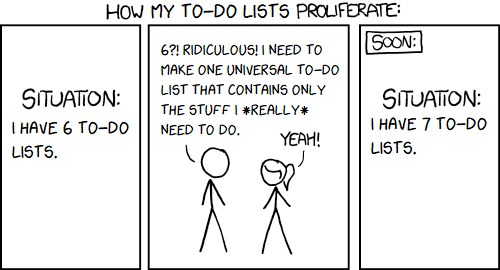
\includegraphics[width=.8\textwidth]{bilder/xkcd_todolist.png}
\end{figure}
